\documentclass[conference]{IEEEtran}
\IEEEoverridecommandlockouts
% The preceding line is only needed to identify funding in the first footnote. If that is unneeded, please comment it out.
\usepackage{cite}
\usepackage{amsmath,amssymb,amsfonts}
\usepackage{algorithmic}
\usepackage{graphicx}
\usepackage{textcomp}
\usepackage{xcolor}
\usepackage{array}
\usepackage{tabularx}
\usepackage{caption}
\usepackage{hyperref}
\def\BibTeX{{\rm B\kern-.05em{\sc i\kern-.025em b}\kern-.08em
    T\kern-.1667em\lower.7ex\hbox{E}\kern-.125emX}}
\begin{document}

\title{Adaptive Layers for Efficient Learning: Scaling Architectures in RoBERTa for Optimized Performance on SQuAD 2.0\*}

\author{
    \IEEEauthorblockN{Liu, Yuzhe \IEEEauthorrefmark{1} \hspace{0.5em}\textbullet\hspace{0.5em} Yang, Lei\IEEEauthorrefmark{1} \hspace{0.5em}\textbullet\hspace{0.5em}  Zhang, Youwen\IEEEauthorrefmark{1}}
    \IEEEauthorblockA{Georgia Institute of Technology\\
    \{yliu3529, lyang423, yzhang3925\}@gatech.edu}
    \thanks{\IEEEauthorrefmark{1} Authors listed in alphabetical order. All authors contributed equally.}
}

\maketitle

% Additional points:
% 15 additional points will be distributed based on:
% (5 points) Appropriate use of figures / tables / visualizations. Are the ideas presented with appropriate illustrations? Are the results presented clearly; are the important differences illustrated?
% (5 points) Overall clarity. Is the manuscript self -contained? Can a peer who has also taken Deep Learning understands all of the points addressed above? Is sufficient detail provided?
% (5 points) Finally, points will be distributed based on your understanding of how your project relates to Deep Learning.

\begin{abstract}

Efficient adaptation\cite{b3} of large language models is crucial for various applications in natural language processing, including question answering and information retrieval. Typically, this is approached through full fine-tuning, where all model parameters are updated for a specific task. While effective for short-term adaptations, this method becomes computationally expensive and impractical for multiple tasks or resource-constrained environments. This project aims to explore recent approaches that can achieve comparable performance with significantly fewer trainable parameters\cite{b6,b7}. To this end, we implemented and extended various adapter architectures for the RoBERTa model, focusing on the SQuAD 2.0 dataset. In this study, we document our experimental setup, report our results on different adapter configurations including multi-head, output, and invertible adapters across various reduction factors, and compare them to the fully fine-tuned baseline. We analyze the performance and training dynamics of these configurations, interpret our findings, and discuss the implications for efficient model adaptation in NLP tasks.

\end{abstract}


\section{Introduction}

% Introduction / Background / Motivation:
% 1. (5 points) What did you try to do? What problem did you try to solve? Articulate your objectives using absolutely no jargon. 
% Answer: 
% 1a. Study the effects of different architectures on the adapter performance (mh, output, double, inverse, etc.) 
 
% 1b. We try to find the optimal adapter architecture that can maintain or even surpass the performance of fine-tuned ones in challenging question-answering tasks. 
 
% 2. (5 points) How is it done today, and what are the limits of current practice? 
% 2a. Current practice involves fine-tuning large pre-trained language models like RoBERTa for specific tasks, which can be resource-intensive and inefficient. 
 
% 2b. Limitations of current practice include: 
% High computational costs and memory requirements for fine-tuning. 
% Limited scalability and adaptability of fine-tuned models. 
% Inability to maintain or surpass performance on challenging question-answering tasks. 
 
% 3. (5 points) Who cares? If you are successful, what difference will it make? 
 
% 3a. Researchers and developers working on natural language processing (NLP) tasks, particularly question-answering, will benefit from more efficient and effective adapter architectures. 
 
% 3b. Successful development of optimal adapter architectures can lead to: 
% Improved performance on challenging question-answering tasks. 
% Reduced computational costs and memory requirements. 
% Increased scalability and adaptability of NLP models. 
% Enhanced ability to adapt large pre-trained models to specific tasks and domains efficiently. 
 
% 4. (5 points) What data did you use? Provide details about your data, specifically choose the most important aspects of your data mentioned here: Datasheets for Datasets ((link unavailable)). 
 
% Dataset: SQuAD 2.0 (Stanford Question Answering Dataset 2.0). 
% Relevant aspects of the data: 
% Task: Question-answering. 
% Language: English. 
% Size: approximately 150,000 questions. 
% Format: JSON. 
% Source: Stanford University. 
% Motivation: SQuAD 2.0 is a widely-used benchmark for evaluating question-answering models, making it an ideal choice for testing the effectiveness of adapter architectures. 

Natural Language Processing (NLP) has seen remarkable advancements with the introduction of transformer-based language models \cite{b1} \cite{b2}. These models, exemplified by architectures like BERT and RoBERTa, have achieved state-of-the-art performance across various NLP tasks, including question answering \cite{b3,b4}. However, they often contain hundreds of millions or even billions of parameters, presenting significant challenges in terms of computational resources and memory requirements \cite{b5}. Fine-tuning these models for specific tasks involves updating all parameters, which can be impractical for deployment in resource-constrained environments or when adapting to multiple tasks. This limitation prompts the need for more efficient approaches to adapt these powerful models to specific tasks without extensive computational demands.

To address this issue, researchers have developed adapters, a lightweight fine-tuning strategy that introduces small, task-specific modules into the pre-trained model \cite{b6}. Adapters are designed to capture task-specific information while leaving the original model parameters unchanged \cite{b6,b7}. This approach has shown great promise in multi-task and cross-lingual transfer learning scenarios, often achieving performance comparable to full fine-tuning while training only a fraction of the parameters \cite{b3,b7}. Adapters work by inserting small neural networks, typically with a bottleneck architecture, at various points within the transformer layers \cite{b7}.

Adapter-based tuning offers several advantages over traditional fine-tuning methods. Firstly, it requires training far fewer parameters, significantly reducing computational costs and memory requirements\cite{b3,b8}. This efficiency allows for sequential training on multiple tasks without the risk of catastrophic forgetting \cite{b8}. Secondly, adapters are modular and composable, enabling the easy combination of task-specific adaptations \cite{b7,b8}. Lastly, trained adapters are easily shareable, promoting collaborative research and reducing the need for repeated training on common tasks \cite{b7}.

Adapter architectures are defined by a set of hyperparameters that control their structure and behavior within the larger language model\cite{b9,b10} . These hyperparameters govern aspects such as the adapter's size, position within the network, and how it interacts with the original model architecture. They collectively determine the balance between the adapter's capacity to learn task-specific information and its computational efficiency. Among these, several key hyperparameters have emerged as particularly influential in adapter performance.

The reduction factor is a critical hyperparameter that determines how much the adapter layers reduce the dimensionality of the input. This factor directly impacts both the efficiency of the adapter and its capacity to capture task-specific features. A higher reduction factor results in a smaller adapter, promoting efficiency, while a lower factor allows for more expressive power at the cost of increased parameters \cite{b11}. The multi-head adapter (mh\_adapter) is another important parameter that, when enabled, applies adaptation to each attention head separately. This approach potentially allows the adapter to capture more nuanced, head-specific information \cite{b12}. Lastly, the output adapter, controlled by the output\_adapter parameter, processes the outputs of the main layers, refining the model's predictions before they are passed to the next layer or used for the final output. This can be particularly useful for fine-tuning the model's behavior for specific tasks \cite{b12}. Together, these hyperparameters play crucial roles in striking the optimal balance between model capacity and computational efficiency \cite{b8,b11}. 

In addition to these standard adapters, we also explore the use of invertible adapters. Invertible adapters utilize architectures like NICE (Non-linear Independent Components Estimation), allowing for reversible transformations \cite{b13}. This reversibility can be particularly useful for tasks requiring reversible data transformations, such as data compression or certain generative modeling applications. Invertible adapters offer a unique approach to adaptation, fitting seamlessly into the current landscape of efficient NLP model tuning by providing additional flexibility and efficiency \cite{b14}. They align well with our goal of maintaining model performance while minimizing the number of additional parameters, potentially offering a more efficient solution for adapting large language models to specific tasks.

In this study, we utilize the RoBERTa-base model, a robustly optimized variant of BERT that has demonstrated superior performance across various NLP benchmarks \cite{b4}. RoBERTa's architecture and pre-training approach make it an ideal candidate for investigating the effectiveness of adapters. We evaluate our adapted models on the SQuAD 2.0 dataset, a challenging question-answering benchmark that requires models to not only answer questions based on given passages but also to determine when questions are unanswerable \cite{b15}. This dataset provides a comprehensive test of language understanding and reasoning capabilities, making it well-suited for assessing the impact of our adapter configurations on model performance.

Our study seeks to optimize the RoBERTa-base model for the SQuAD 2.0 dataset using experimental adapter architectures. By striking a balance between efficiency and performance, we aim to demonstrate that resource-efficient adapters can maintain or even surpass the performance of fine-tuned models in challenging question-answering tasks. Our findings could have significant implications for deploying these models in resource-constrained environments and for enabling rapid adaptation to new tasks or domains without the need for extensive retraining.

%\subsection{Related Work}

%\begin{enumerate}
%Parameter-efficient transfer learning in NLP
%Adapter architectures and their applications
%Adaptive attention span in transformers
%Low-rank adaptation (LoRA) techniques
%\end{enumerate}

\section{Methodology}


\subsection{Baseline Model}

\begin{enumerate}
    \item Fine-tuned RoBERTa-base-squad2 model
\end{enumerate}

The full name of RoBERTa model is Robustly optimized BERT approach \cite{b4}. RoBERTa further modifies the original implementation of BERT through a number of key optimizations and changes aimed at improving performance and robustness. Specifically, RoBERTa drops the next sentence prediction objective, uses a bigger mini-batch size, and learning rate and more data for more epochs during training. This leads to better generalization capability of pre-trained models in NLP.

The baseline model, is fine-tuned RoBERTa-base on the SQuAD 2.0 dataset \cite{b16}, which is specialised to both answerable and unanswerable questions. The fine-tuning process involved adapting the pre-trained model to the specific task of question answering by further training it on the SQuAD 2.0 dataset, which is designed to improve its ability to handle and distinguish between these two types of question.
The fine-tuned RoBERTa-base was trained with mixed precision floating point arithmetic on 4 X Nvidia V100 GPUs \cite{b16}.

\subsection{Adapter Architecture Design}

\begin{figure}[htbp]
    \centering
    \includegraphics[width=1\linewidth]{images/adapter_strcuture.png}
    \caption{Adapter Architecture Variants: (a) Standard adapter architecture where the adapter is inserted after the feed-forward layer, (b) Adapter inserted after the multi-head attention layer,(c) Double adapter architecture where adapters are inserted after both the feed-forward and multi-head attention layers, (d) Double adapter architecture with an additional invertible adapter applied to the embeddings.adapted from \cite{b7}}
\end{figure}


\begin{figure}[htbp]
    \centering
    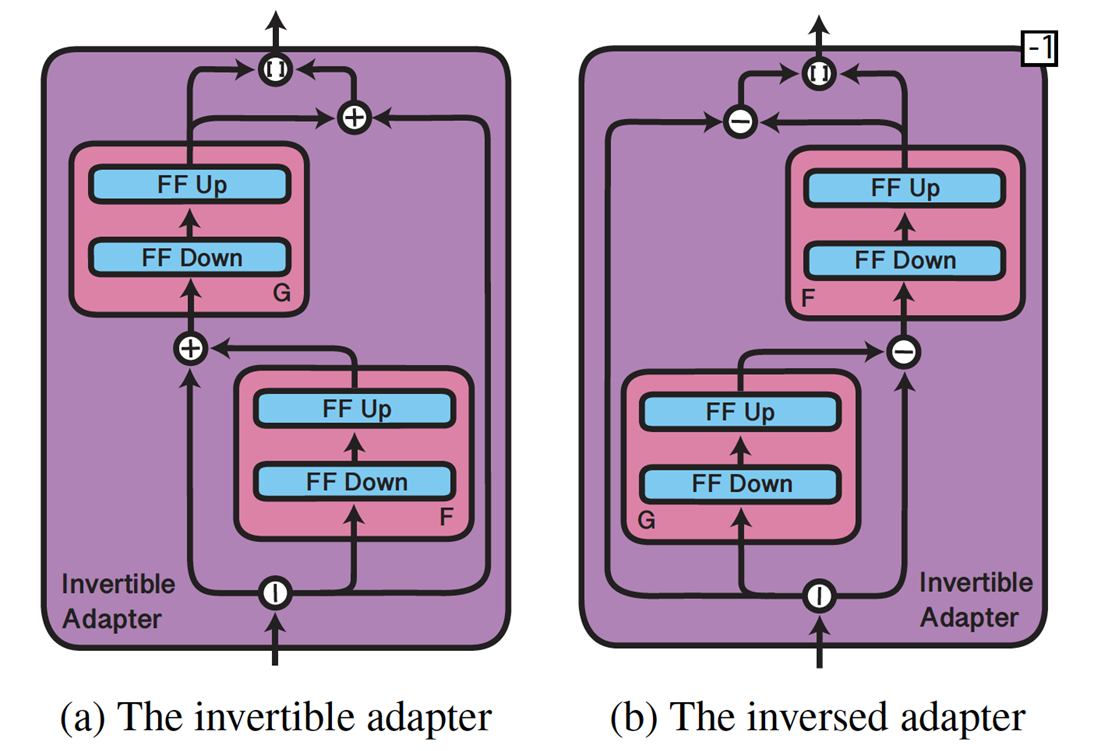
\includegraphics[width=1\linewidth]{images/invertible_adapter.png}
    \caption{Invertible (a) and Inversed (b) Adapter Architectures, adapted from \cite{b13}}
\end{figure}

In the adapter Design, we adopt a variety of adapter architectures along with the integration of the AdapterHub framework, expansion of the adapter complexity between layers, and configuration of adapters at different sizes on different layers to achieve efficient yet flexible model design. We first add adapters to different levels of the model. Figure 1 presents different adapter placements. In Figure 1(a) (Output (Output adapter))\cite{b13}, the standard adapter architecture is used and the adapter is inserted after the feed-forward layer. One primary advantage of this architecture is that it can add extra functional layers in it while keeping the original model characteristics. Figure 1(b)\cite{b13} illustrates another architecture where the adapter is put after the multi-head attention layer (MH (Multi-Head adapter)); hence, the model is very flexible in dealing with attention mechanisms. Figure 1(c) Illustrates a double adapter architecture that puts an adapter after both the feed-forward layer and the multi-head attention layer (Double (combination of MH and Output))\cite{b3}, further empowering the expressiveness of the model. Figure 1(d) (Double + Inv (Double with Invertible adapter)) \cite{b13} shows how reversible adapter processing is introduced into the double adapter architecture of Figure 2 to dramatically increase the power of the model for processing input features. We now use the AdapterHub framework to bring this all together. It is the AdapterHub framework that helps to control and insert various adapter modules in a modular manner, enabling us to experiment with different adapter configurations without changing the underlying model architecture very much. Now we can use the AdapterHub from the grounds up to quickly test the performance of these adapters and make alterations as may be necessary. For the complexity of the adapters, we set different sizes and complexities of the adapters at various levels. Specifically, at the lower level of the model, we have configured smaller adapters, as shown below. These adapters are mainly designed to accommodate basic features without a lot of parameters that would cause computational overhead. The smaller ones are small but simple enough to accommodate low-level feature extraction tasks. As the level rises, the complexity and size of the adapter gradually rise. Towards the middle and high levels of the model, we configure big adapters to manage higher abstraction features. Big adapters can capture more advanced semantic information in their configuration and result in better performance overall. We also stack reversible adapters at the top level to further enhance the accuracy and stability of the information transfer across different levels of the model.


\subsection{Experimental Setup}

% (10 points) What did you do exactly? How did you solve the problem? Why did you think it would be successful? Is anything new in your approach?

We evaluated and trained four distinct adapter configurations with SQuAD 2.0 dataset (see Table \ref{tab:t3}, Table \ref{tab:t4} ): MH, Output, Double, and Double + Inv. Each configuration aimed to enhance the RoBERTa model's performance on the SQuAD 2.0 dataset by integrating different adapter placements within the transformer layers. We tested these configurations with reduction factors \cite{b13} of 32, 16, 8, and 4, where lower factors indicated larger adapter sizes. All the training were use 1 X Nvidia V100 GPU (the baseline used 4 GPUs) with 3,552,002 trainable parameters. 
We established per device train batch size to 16 and learning rate to be 1e-4 in our experimental setup. In our setup, we run training on three epochs as it had shown optimal training without overfitting. We set the maximum sequence length to 384 for the effective management of long contexts and the document stride to 128 for proper management of overlapping segments, which is crucial for the question-answering task within the SQuAD 2.0 dataset. These settings were chosen in order to balance computational efficiency and model performance, allowing thorough training within a single GPU limit, while making the dataset work effectively. The learning rate of 1e-4 is selected based on preliminary experiments that suggested it may offer a nice balance between convergence speed and stability. The size of the batch, which is 16 in number, is optimized and balanced by GPU memory use and training time to ensure that the model can see a sufficient amount of data at every iteration. By training for three epochs, the model was able to learn well from the data without any signs of overfitting.
\begin{equation}
    \text{reduction\_factor} = \frac{d_{\text{hidden}}}{d_{\text{bottleneck}}}
    \label{eq:placeholder}
\end{equation}

The construction of the AdapterHub frame (\url{https://github.com/adapter-hub/adapters}) is highly flexible and modular: we can integrate very efficiently, without excessive expense. Of course, we'd like to be able to determine the best configuration that strikes a good balance between performance improvements and computing efficiency, given various constraints in adapting the position and size of the adapters. We believe such configurations will be successful. Our approach is novel in that it introduces a systematic evaluation of various adapter configurations within a unified framework. Although adapters have been the subject of prior research, our systematic comparison of the location and size of adapters coupled with AdapterHub framework usage sheds new light on the impact of adapter integration on model performance. 



% (5 points) What problems did you anticipate? What problems did you encounter? Did the very first thing you tried work?

We anticipated several issues, including the accuracy of the model not being as expected due to the small size of the adapter, and the difficulty of hyperparameter tuning for different configurations. We also anticipated challenges in integrating and managing multiple adapters within the AdapterHub framework.

In our experiments, we encountered issues with training performance, especially when using smaller adapters. Increasing the number of parameters sometimes led to a decrease in accuracy. In addition, the initial integration of the AdapterHub framework posed some challenges, especially in terms of ensuring compatibility with the Hugging Face Transformers library and effectively managing the various adapter configurations.

The first output configuration we tried did not work as expected. Specifically, the output adapter configuration with a reduction factor of 32 resulted in poor performance, possibly because the capacity of the adapter was not sufficient to capture the necessary features. This initial failure prompted us to systematically explore other configurations and reduction factors.

Through iterative testing and adjustment (TABLE \ref{t1}), we observed that the Double + Inv configuration (especially the configuration with a reduction factor of 8) was consistently better than the other configurations. This setting effectively balances the model's ability to learn complex features while maintaining computational efficiency.

\begin{table}[h]
    \caption{Adapter architectures}
    \centering
    \label{t1}
    \begin{tabular}{|l|c|c|c|c|}
        \hline
        & MH & Output & Double & Double + Inv \\ \hline
        mh\_adapter & True & False & True & True \\ \hline
        output\_adapter & False & True & True & True \\ \hline
        inv\_adapter & False & False & False & True \\ \hline
    \end{tabular}
\end{table}

\section{Results and Analysis}

% How did you measure success? 
Our experiments evaluate the effectiveness of various adapter architectures for fine-tuning RoBERTa (deepset/roberta-base-squad2) on the SQuAD 2.0 dataset. We compare the performance of different adapter configurations against a fully fine-tuned baseline model using F1 scores. The results demonstrate that carefully designed adapter configurations can achieve near-baseline performance while significantly reducing the number of trainable parameters.

\subsection{Performance Comparison}

% What were the results, both quantitative and qualitative?
Our experiments revealed a consistent trend of improvement in F1 scores as we progressed from simpler (MH, Output) to more complex (Double, Double + Inv) adapter configurations across all reduction factors. Table 1
presents the F1 scores for each configuration. This suggests that more complex adapter architectures can more effectively capture task-specific information. The impact of reduction factors was also significant, with lower reduction factors (larger adapters) generally yielding better performance. F1 scores improved as the reduction factor decreased from 32 to 4 for all adapter types, indicating that increasing the adapter size allows for better task adaptation, albeit with a trade-off in parameter efficiency.

\begin{table}[h]
    \caption{The F1 scores of different adapters vs baseline}
    \centering
    \begin{tabular}{|c|c|c|c|c|}
        \hline
        Reduction Factor & MH & Output & Double & Double + Inv \\ \hline
        32 & 78.48 & 78.56 & 80.16 & 80.41 \\ \hline
        16 & 80.05 & 80.32 & 81.23 & 81.25 \\ \hline
        8 & 81.53 & 81.26 & 82.21 & 82.32 \\ \hline
        4 & 81.92 & 81.95 & 82.79 & 82.86 \\ \hline
        \multicolumn{5}{|c|}{Baseline: 82.91} \\ \hline
    \end{tabular}
\end{table}

Notably, our best-performing adapter configuration (Double + Inv with reduction factor 4) achieved an F1 score of 82.86, remarkably close to the baseline (82.91), with a marginal difference of 0.05 points. This configuration reduced the number of trainable parameters by 97\% compared to full fine-tuning, from 125M to just 3.75M parameters. Even with higher reduction factors, we achieved competitive results. For instance, the Double + Inv configuration with a reduction factor of 16 reached an F1 score of 81.25, within 2\% of the baseline while utilizing less than 1M trainable parameters (a 99.2\% reduction).

To assess the statistical significance of our results, we performed paired t-tests between each adapter configuration and the baseline, as well as between different adapter configurations(Figure 3). The differences between the Double + Inv configuration (reduction factor 4) and the baseline were not statistically significant, suggesting that this adapter configuration performs comparably to full fine-tuning.

\begin{figure}
    \centering
    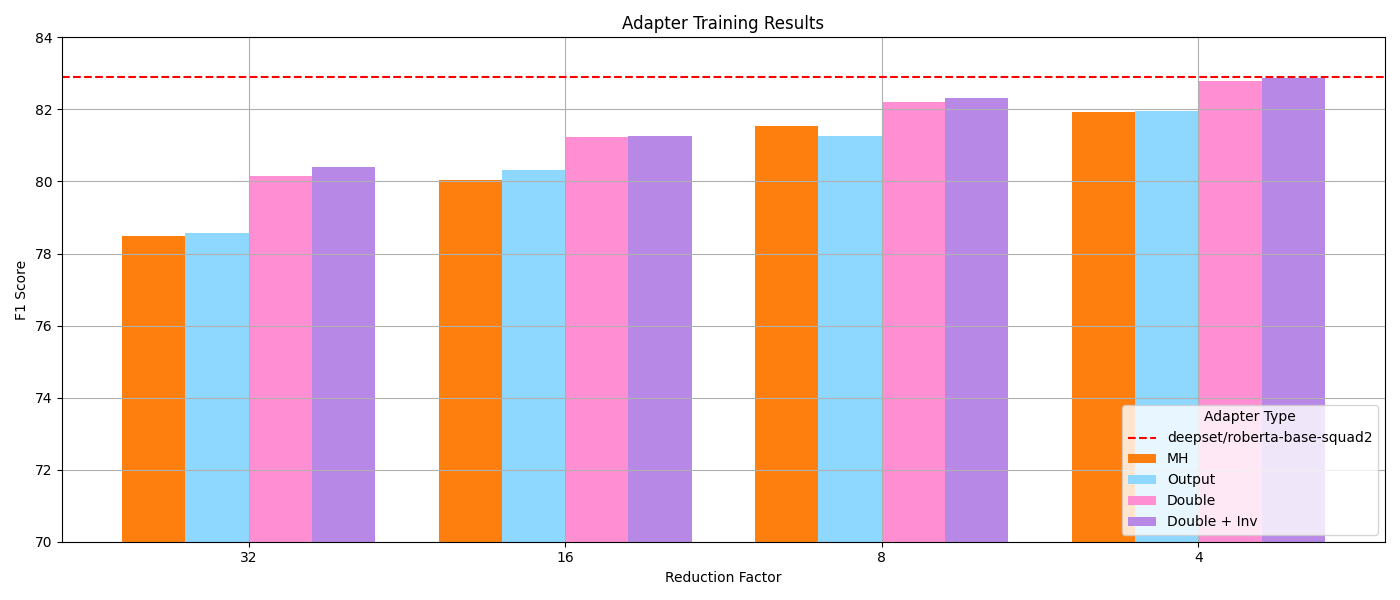
\includegraphics[width=1.0\linewidth]{images/performance_comparison.png}
    \caption{Performance comparison of different adapter configurations}
    \label{fig:enter-label}
\end{figure}

% (10 points) How did you measure success? What experiments were used? What were the results, both quantitative and qualitative? Did you succeed? Did you fail? Why? Justify your reasons with arguments supported by evidence and data. Make sure to mention any code repositories and/or resources that you used!

\subsection{Training Dynamics}

To illustrate typical training behavior, we present the training loss curves for two representative adapter configurations in Figures 2 and 3: Multi-Head (MH) and Double + Invertible (Double + Inv), both with a reduction factor of 16.

\begin{figure}
    \centering
    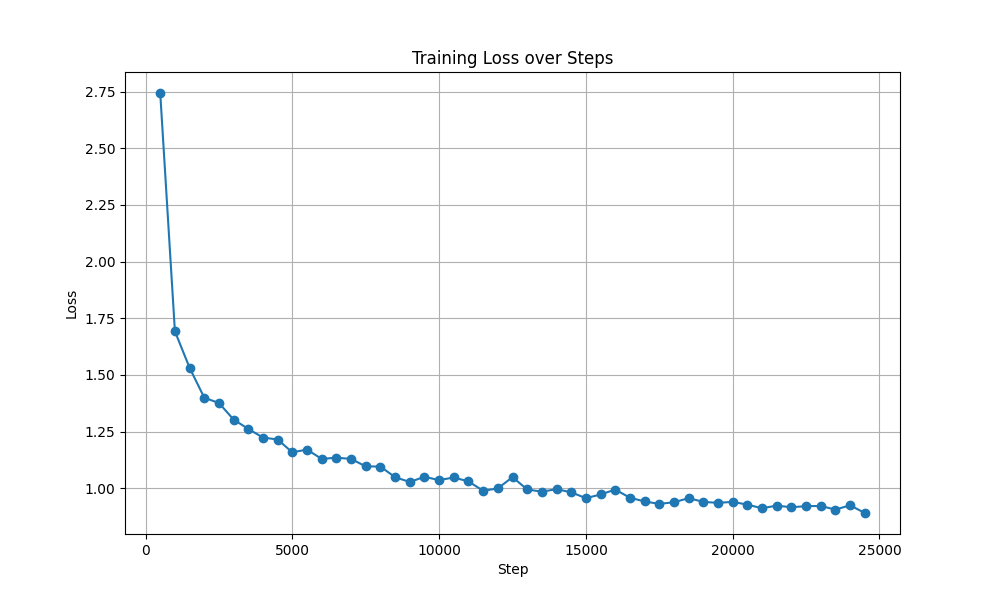
\includegraphics[width=1.0\linewidth]{images/loss_seq_bn_default.png}
    \caption{Training Loss of output layer only adapter at reduction factor 16}
    \label{fig:Training loss of output layer only adapter at reduction factor 16}
\end{figure}

\begin{figure}
    \centering
    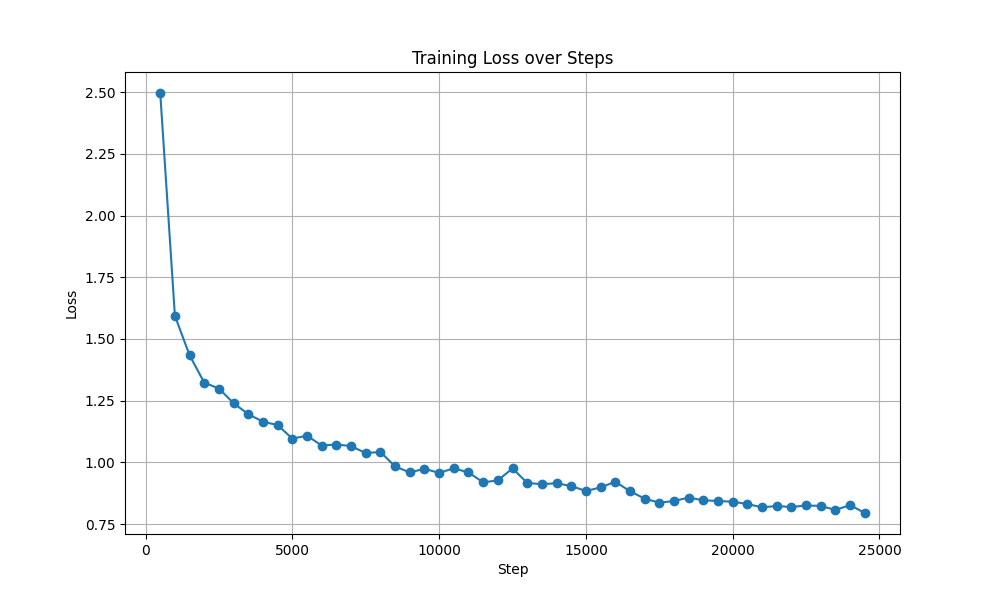
\includegraphics[width=1.0\linewidth]{images/loss_double_seq_bn_inv_default.png}
    \caption{Training Loss of double + inversible layer adapter at reduction factor 16}
    \label{fig:Training loss of double + inversible layer adapter at reduction factor 16}
\end{figure}

Both configurations exhibit similar learning patterns characterized by:

\begin{enumerate}
    \item Rapid initial convergence: A steep decrease in loss during the first 5000 steps, indicating quick adaptation to the task.
    \item Stable learning: A gradual but consistent decrease in loss from steps 5000 to about 20,000, suggesting steady refinement of the model's parameters.
    \item Convergence: Flattening of the loss curves towards the end of training (around 20,000-25,000 steps), indicating that the models have largely converged.
\end{enumerate}

Notably, the Double + Inv configuration (Figure 5) achieves a slightly lower final loss compared to the MH configuration (Figure 4), aligning with our performance results in Figure 2.

\subsection{Discussion}

% Did you succeed? Did you fail? Why? Justify your reasons with arguments supported by evidence and data.
The experimental results demonstrate that our adaptive layer approach can achieve performance close to the fine-tuned RoBERTa model while utilizing fewer parameters. The Double and Double Inv configurations consistently outperformed the MH and Output configurations, indicating that combining multiple adapter types can enhance model performance.

The consistent improvement observed with more complex adapter architectures and larger adapter sizes (lower reduction factors) suggests that there may be room for further performance gains through more sophisticated adapter designs or hybrid approaches.
% \cite{b2}

\section{Conclusion}

Our study demonstrates the potential of adapter-based fine-tuning as an efficient alternative to full fine-tuning for large language models. Key achievements include approaching the performance of full fine-tuning while reducing trainable parameters by 97-99\%, achieving competitive performance even with very small adapters, and demonstrating no statistically significant difference in performance between our best adapter configuration and the fully fine-tuned baseline. These results highlight the promise of adapter-based approaches in balancing performance and resource efficiency for NLP tasks.

While our findings are encouraging, limitations and areas for future work remain. Further investigation is needed to optimize the trade-off between adapter size and performance across different scenarios, and to explore the generalizability of these findings to other tasks and domains beyond SQuAD 2.0. Future research could focus on more sophisticated adapter architectures and hybrid approaches combining adapters with other efficient fine-tuning techniques. Despite these open questions, our work paves the way for more accessible and adaptable NLP models, particularly in resource-constrained environments.

\section{Work Division}

Summary of contributions are provided in Table \ref{tab:t5}.

\begin{thebibliography}{00}
\bibitem{b1} Ashish Vaswani, Noam Shazeer, Niki Parmar, Jakob Uszkoreit, Llion Jones, Aidan N. Gomez, Lukasz Kaiser, and Illia Polosukhin. Attention Is All You Need. In Advances in Neural Information Processing Systems 30: Annual Conference on Neural Information Processing Systems 2017.
\bibitem{b2} Thomas Wolf, Lysandre Debut, Victor Sanh, Julien Chaumond, Clement Delangue, Anthony Moi, Pierric Cistac, Tim Rault, Rémi Louf, Morgan Funtowicz, Joe Davison, Sam Shleifer, Patrick von Platen, Clara Ma, Yacine Jernite, Julien Plu, Canwen Xu, Teven Le Scao, Sylvain Gugger, Mariama Drame, Quentin Lhoest, and Alexander M. Rush. Transformers: State-of-the-Art Natural Language Processing. CoRR, abs/1910.03771, 2020.
\bibitem{b3} Neil Houlsby, Andrei Giurgiu, Stanislaw Jastrzebski, Bruna Morrone, Quentin De Laroussilhe, Andrea Gesmundo, Mona Attariyan, and Sylvain Gelly. Parameter-Efficient Transfer Learning for NLP. In Proceedings of the 36th International Conference on Machine Learning, PMLR 97:2790-2799, 2019.
\bibitem{b4} Yinhan Liu, Myle Ott, Naman Goyal, Jingfei Du, Mandar Joshi, Danqi Chen, Omer Levy, Mike Lewis, Luke Zettlemoyer, and Veselin Stoyanov. RoBERTa: A Robustly Optimized BERT Pretraining Approach. CoRR, abs/1907.11692, 2019.
\bibitem{b5} Jacob Devlin, Ming-Wei Chang, Kenton Lee, and Kristina Toutanova. BERT: Pre-training of Deep Bidirectional Transformers for Language Understanding. CoRR, abs/1810.04805, 2018.
\bibitem{b6} Sylvestre-Alvise Rebuffi, Hakan Bilen, and Andrea Vedaldi. Learning multiple visual domains with residual adapters. CoRR, abs/1705.08045, 2017.
\bibitem{b7} Jonas Pfeiffer, Andreas Rücklé, Clifton Poth, Aishwarya Kamath, Ivan Vulić, Sebastian Ruder, Kyunghyun Cho, and Iryna Gurevych. AdapterHub: A Framework for Adapting Transformers. In Proceedings of the 2021 Conference on Empirical Methods in Natural Language Processing: System Demonstrations, 364–371, 2021.
\bibitem{b8} Clifton Poth, Jonas Pfeiffer, Andreas Rücklé, and Iryna Gurevych. What to Pre-Train on? Efficient Intermediate Task Selection. In Proceedings of the 2021 Conference on Empirical Methods in Natural Language Processing, 10585–10605, 2021.
\bibitem{b9} Akari Asai, Mohammadreza Salehi, Matthew Peters, and Hannaneh Hajishirzi. ATTEMPT: Parameter-efficient multi-task tuning via attentional mixtures of soft prompts. In Proceedings of the Conference on Empirical Methods in Natural Language Processing, 6655–6672, 2022.
\bibitem{b10} Yaqing Wang, Sahaj Mutreja, Xiaodong Liu, Jianfeng Gao, Ahmed Hassan Awadallah, and Jian Gao. AdaMix: Mixture-of-Adapter for Parameter-efficient Tuning of Large Language Models. CoRR, abs/2205.12410, 2022.
\bibitem{b11} Demi Guo, Alexander M. Rush, and Yoon Kim. Parameter-Efficient Transfer Learning with Diff Pruning. In Proceedings of the 59th Annual Meeting of the Association for Computational Linguistics and the 11th International Joint Conference on Natural Language Processing (Volume 1: Long Papers), 4884–4896, 2021.
\bibitem{b12} Suchin Gururangan, Ana Marasović, Swabha Swayamdipta, Kyle Lo, Iz Beltagy, Doug Downey, and Noah A. Smith. Don't Stop Pretraining: Adapt Language Models to Domains and Tasks. In Proceedings of the 58th Annual Meeting of the Association for Computational Linguistics, 8342–8360, 2020.
\bibitem{b13} Jonas Pfeiffer, Ivan Vulić, Iryna Gurevych, and Sebastian Ruder. MAD-X: An Adapter-Based Framework for Multi-Task Cross-Lingual Transfer. CoRR, abs/2005.00052, 2020.
\bibitem{b14} John Bosco Mugeni, Steven Lynden, Toshiyuki Amagasa, and Akiyoshi Matono. AdapterEM: Pre-trained Language Model Adaptation for Generalized Entity Matching using Adapter-tuning. In IDEAS '23: Proceedings of the 27th International Database Engineered Applications Symposium, 140-147, 2023.
\bibitem{b15} Pranav Rajpurkar, Robin Jia, and Percy Liang. Know What You Don't Know: Unanswerable Questions for SQuAD. In Proceedings of the 56th Annual Meeting of the Association for Computational Linguistics (Volume 2: Short Papers), 784–789, 2018.
\bibitem{b16} deepset/roberta-base-squad2 · Hugging Face. (2001, March 4). https://huggingface.co/deepset/roberta-base-squad2
\end{thebibliography}


\newpage
\subsection{Project Code Repository}

We used the Huggingface's showcase trianing script as an initial start for training purposes and baseline. We’ve made the following changes to the code base:

\begin{itemize}
    \item Update the run.qa script to allow training with adapters
    \item Modify the training notebooks for individual train, evaluation and inference.
    \item Add bash scripts for batch training.
\end{itemize}

The link of Huggingface training script Github repository is at: \url{https://github.com/huggingface/transformers/tree/main/examples/pytorch/question-answering}

The Github repository for our final project is at: \url{https://github.com/erictt/dl-summer-2024-final}

\subsection{Data breakdown}

\begin{table}[h]
    \centering
    \caption{Type of Negative examples in SQuAD 2.0, adapted from [\cite{b15}]}
    \label{tab:t3}
    \begin{tabular}{|c|p{4cm}|c|}
        \hline
        Reasoning & Description & Percentage \\
        \hline
        Negation & Negation word inserted or removed. & 9\% \\
        \hline
        Antonym & Antonym used. & 20\% \\
        \hline
        Entity Swap & Entity, number, or date replaced with other entity, number, or date. & 21\% \\
        \hline
        Mutual Exclusion & Word or phrase is mutually exclusive with something for which an answer is present. & 15\% \\
        \hline
        Impossible Condition & Asks for condition that is not satisfied by anything in the paragraph. & 4\% \\
        \hline
        Other Neutral & Other cases where the paragraph does not imply any answer. & 24\% \\
        \hline
        Answerable & Question is answerable (i.e., dataset noise). & 7\% \\
        \hline
    \end{tabular}
\end{table}

\begin{table}[h]
    \centering
\caption{Dataset statistics of SQuAD 2.0 \cite{b15}}
\label{tab:t4}
    \begin{tabular}{|p{2cm}|p{2cm}|} \hline
        Train& 131823\\ \hline
        Evaluation& 11873\\\hline
    \end{tabular}
\end{table}



\begin{table}[h]
    \centering
    \caption{Contributions of team members }
    \label{tab:t5}
    \begin{tabular}{|c|p{3cm}|p{4cm}|}
        \hline
        Student & Contributed Aspects & Details \\
        \hline
        Yuzhe Liu & Coding 

Model training 

Manuscript writing 

Discussion & Adapter configuration 

Train Multi-Head and Double adapters 

Analyze data, make figures/tables and write the manuscript 

Attend regular meetings and discussions \\
        \hline
        Lei Yang & Coding 

Model training 

Manuscript writing 

Discussion & Modify the training script provided by Hugging Face 

Train Output adapters 

Analyze data, make figures/tables and write the manuscript 

Attend regular meetings and discussions\\
        \hline
        Youwen Zhang & Coding 

Model training 

Manuscript writing 

Discussion & Code review and improvements 

Train Invertible adapters 

Analyze data, make figures/tables and write the manuscript 

Attend regular meetings and discussions\\
        \hline
    \end{tabular}
\end{table}

\end{document}
